% https://www.wikiwand.com/en/Sobel_operator
% https://www.scss.tcd.ie/~munnellg/projects/edge_detection.html
% https://sbme-tutorials.github.io/2018/cv/notes/4_week4.html#edge-detection-kernels

Combinada -> Modulo gradiente, gradiente x e y

+ Edge detection

\begin{figure}[H]
    \centering
    \begin{subfigure}{0.4\textwidth}
        \centering
        \begin{kmatrix}
    \matrix[square matrix]{
        -1 & 0 & 1 \\
        -2 & 0 & 2 \\
        -1 & 0 & 1 \\
    };
\end{kmatrix}
        \caption{~$h_3$}
        \label{fig:h3}
    \end{subfigure}%
    \begin{subfigure}{0.4\textwidth}
        \centering
        \begin{kmatrix}
    \matrix[square matrix]{
        -1 & -2 & -1 \\
        0 & 0 & 0 \\
        1 & 2 & 1 \\
    };
\end{kmatrix}
        \caption{~$h_4$}
        \label{fig:h4}
    \end{subfigure}

    \caption{??}
    \label{fig:sobel:kernel}
\end{figure}

\begin{figure}[H]
    \centering
    \begin{subfigure}{0.48\textwidth}
        \centering
        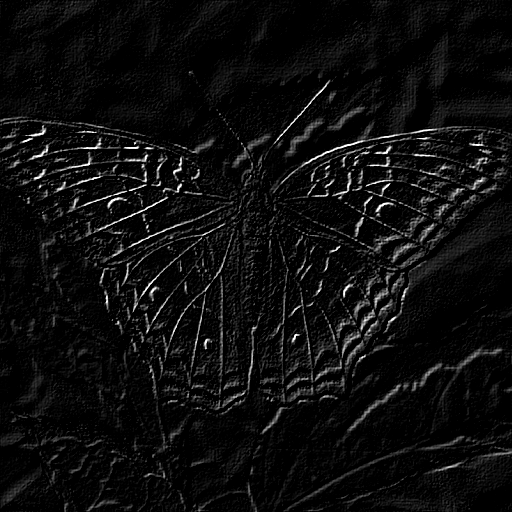
\includegraphics[width=0.9\textwidth]{imagens/butterfly.png}
        \caption{Original: \texttt{butterfly.png}.}
    \end{subfigure}%
    \begin{subfigure}{0.48\textwidth}
        \centering
        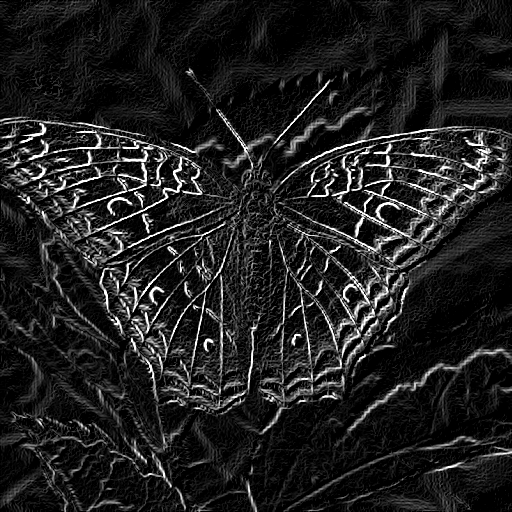
\includegraphics[width=0.9\textwidth]{resultados/butterfly_h3h4.png}
        \caption{Convolução com $h_3$ e $h_4$.}
    \end{subfigure}\\[8pt]
    \begin{subfigure}{0.48\textwidth}
        \centering
        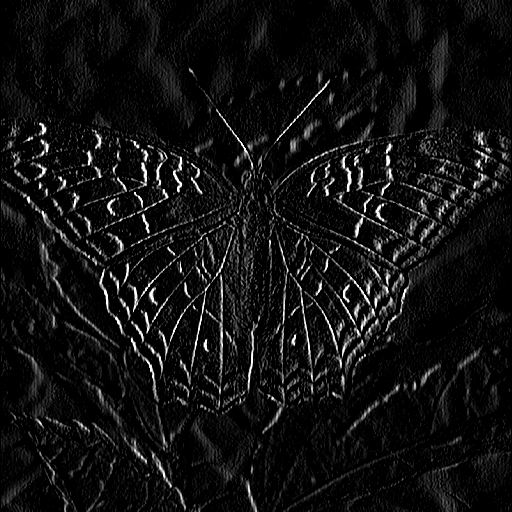
\includegraphics[width=0.9\textwidth]{resultados/butterfly_h3.png}
        \caption{Convolução com $h_3$.}
    \end{subfigure}%
    \begin{subfigure}{0.48\textwidth}
        \centering
        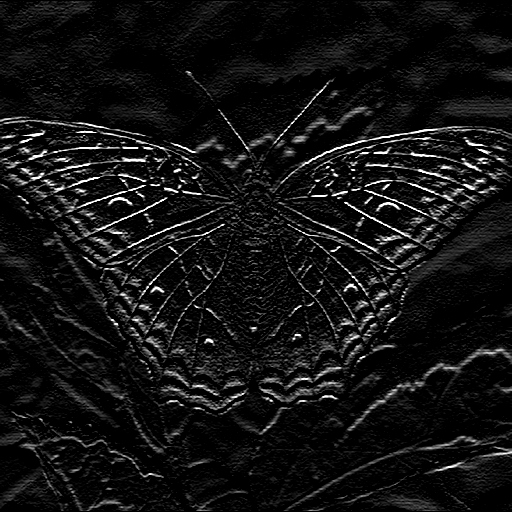
\includegraphics[width=0.9\textwidth]{resultados/butterfly_h4.png}
        \caption{Convolução com $h_4$.}
    \end{subfigure}

    \caption{??}
\end{figure}
